\chapter{Prototypers påverkan på utveckling av användargränssnitt av Rebecca Lindblom}
\section{Introduktion}
\label{cha:rebecca-introduction}
Att skapa prototyper kan i vissa människors ögon vara ett tidskrävande och onödigt moment som hindrar utvecklingen i ett mjukvaruprojekt från att komma igång. Men prototyper är också ett kraftfullt verktyg för att få fram information och hitta snabbare vägar som annars inte hade upptäckts i ett projekt. 

\subsection{Syfte}
\label{sec:rebecca-purpose}
Syftet med denna studie är att undersöka skillnaderna mellan att ha och att inte ha prototyper som underlag för utvecklingen av användargränssnitt. Studien undersöker hur en grupp har upplevt arbetet med och utan prototyper, och om dessa prototyper har underlättat utvecklingsarbetet, samt gruppens förmåga att komma överens i designbeslut.

\subsection{Frågeställningar}
\label{sec:rebecca-research-questions}
De frågeställningar som undersöks är:
\begin{enumerate}
	\item Hur kan prototyper förenkla utvecklingsarbetet för en grupp?
	\item Hur kan prototyper underlätta för gruppen att komma överens?
	\item Kan prototyper spara tid i utvecklingsarbetet?
\end{enumerate}

\subsection{Avgränsningar}
\label{sec:rebecca-delimitations}
Studien kommer endast baseras på detta kandidatarbete som utförs i kursen TDDD96 på Linköpings universitet våren 2017. 
\\ \\
Prototyperna i studien avser endast grafiska representationer av användargränssnitt och tar därför inte prototyper för andra delar av system i beaktande. Studien undersöker även endast hur de befintliga prototyperna har påverkat arbetet och gör ingen skillnad i olika typer av prototyper och dess olika påverkan.

\section{Teori}
\label{cha:rebecca-theory}
Utformning av ett användargränssnitt är en väsentlig del av mjukvaruutveckling. Men denna del kan också skapa meningsskiljaktigheter då en textbaserad beskrivning, från till exempel en kravspecifikation, tenderar att skapa en mental bild hos varje person i arbetsgruppen. Därmed står projektet med lika många versioner av designen som det finns medlemmar i gruppen. \cite{prototyping-guide} %ok
\\ \\
Prototyper har använts långt tillbaka i historien, och använts till många olika saker inom teknisk utveckling. Då definitionen av en prototyp är en mall eller en originalmodell att basera en större tillverkning på, har prototyper följt med den tekniska utvecklingen. Från att ha använts av Leonardo da Vinci när han utforskade vilka av hans idéer som var möjliga att bygga, fram till dagens produktion av digitala verktyg och program. \cite{effective-prototyping} %ok
Denna studie undersöker prototyper för utveckling av användargränssnitt. Grundläggande teori om prototyper finns i avsnitt \ref{sec:prototypes-theory}.

\subsection{Designprocessen}
Designprocessen består av tre faser, konceptfasen, bearbetningsfasen och detaljeringsfasen. %ok
Under konceptfasen görs undersökningar och insamlingar av information för att ta reda på vad de olika aktörerna i projektet tycker är viktigt. Idéer och förslag tas fram utefter den insamlade informationen. %ok
Efter detta går projektet in i bearbetningsfasen där skisser och planering görs för att bestämma hur systemet ska se ut och implementeras. Idéer anpassas för att fungera med den tekniska lösningen. %ok
Detaljer och finslipning sker i detaljeringsfasen, där systemet specificeras noggrant. % ok
\cite{arvolaboken} %ok
\\
\begin{figure}[!htb]
  \centering
  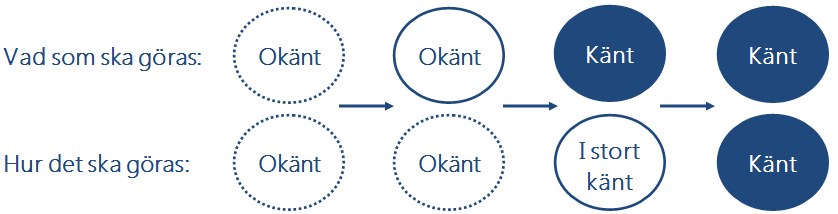
\includegraphics[scale=0.6]{design_process}
  \caption[Illustration över hur designprocessen minskar osäkerheten i ett projekt.]{Illustration över hur designprocessen minskar osäkerheten i ett projekt, fritt efter Arvola \protect\cite{arvolaboken}, s. 8}
  \label{fig:design_process}
\end{figure}
\ \\
Enligt Arvola \cite{arvolaboken} är designprocessen på så sätt en process för att minska osäkerheten i ett projekt. I figur \ref{fig:design_process} representeras de olika faserna i designprocessen av de tre pilarna. Osäkerheten minskar efter varje steg.  %ok

\subsection{Prototyper inom mjukvaruutveckling}
Att arbeta med prototyper kan ske under alla delar av designprocessen, med mer detaljerade sådana desto längre in i processen man kommer. Prototyper med mindre detaljer kallas för LoFi och prototyper med mer detaljer kallas för HiFi. Prototyper kan också ha en blandad detaljeringsgrad och kan då vara mer som skisser för vissa delar av det avbildade systemet och ha mer funktionalitet för andra delar. Prototyper kan ha olika användningsområden i olika delar av ett utvecklingprojekt. \cite{effective-prototyping} %ok
Utvärdering av prototyperna kan ske av arbetsgruppen i samråd med kund, eller genom ett användbarhetstest, och sker genom hela processen, se avsnitt \ref{sec:usability-tests}.
\\ \\
En kravspecifikation kan bli ett väldigt detaljerat och stort dokument desto större ett mjukvaruprojekt blir. Genom att använda prototyper får alla inblandade en mer påtaglig bild över vad det är som faktiskt ska byggas. Prototyperna ger också en bättre helhetsbild till skillnad från endast en kravspecifikation där informationen ges en del i taget per rad. Prototyper visar vad som ska göras istället för att berätta. \cite{prototyping-guide} %ok
Enligt Warfei \cite{prototyping-guide} %ok
gick dennes företag från en kravbaserad process till en prototypbaserad process, och detta ökade överenskommelsen gällande tolkningarna av systemet från 60-80 procent upp till 90 procent. Överenskommelsen leder i sin tur till att mindre arbete behöver göras om, och fel upptäcks tidigt i processen. Detta minimerar i sin tur användningen av resurser och tillhörande risker med ett projekt. \cite{prototyping-guide} %ok
För en utvecklare som arbetat i två veckor med en del av ett system kan det kännas både onödigt och irriterande att behöva kasta bort sitt arbete för att det inte stämde överens med någon annans bild av hur det skulle fungera eller se ut. Känslan av ägande blir mindre desto mindre tid som har lagts på att utvecka ett delsystem. Snabba prototyper blir ett hjälpmedel för utvecklingsteamet att tidigt kasta bort idéer innan en större mängd tid hinner läggas på dem, så att andra bättre idéer istället kan hamna i fokus. \cite{paper-prototyping} %ok

\section{Metod}
\label{cha:rebecca-method}
Som beskrivet i avsnitt \ref{sec:prototypes} togs prototyper fram och användes under projektets gång. Som avsnittet även nämner fanns det för vissa delar av användargränssnittet inte några prototyper som grund för utseendet vid utvecklingen. Vid utveckling av en funktionalitet med en prototyp arbetade utvecklarna för att resultatet så väl som möjligt skulle matcha prototypen. Då det inte fanns en prototyp fanns det inget heller som begränsade utvecklarna i utformningen, och de kunde på så sätt själva välja hur de ville forma funktionaliteten i fråga. Eftersom utvecklarna själva skrev testfallen för testningen av funktionaliteten fanns inte heller där någon spärr för att neka eller acceptera en utvecklad funktionalitet. Först när en testare gick igenom testfallen och såg funktionalitetens utformning kunde denne jämföra resultatet med sin egen interna bild. Därefter handlade det endast om tycke och smak, och det fanns ingen organiserad metod för utvecklarna att få svar på hur resten av gruppen tänkte och ville att funktionaliteten skulle se ut. I vissa fall ritades en pappersprototyp, och i vissa fall valde utvecklarna en helt egen ny design, och processen började på detta sätt om och om igen tills en majoritet av gruppen tyckte att resultatet var bra och på så sätt godkände resultatet.
\\ \\
\begin{table}[h!]
	\caption{Datum för versioner av utvalda delar för jämförelse.}
  \def\arraystretch{1.5}
  \begin{adjustbox}{max width=\textwidth}
    \begin{tabularx}{\textwidth}{ | X | r | r |}
      \hline
      \textbf{Del} & \textbf{Version} & \textbf{Datum} \\
      \hline
      Hjälpruta & 1 & 2017-03-30 \\
      \hline
      Hjälpruta & 2 & 2017-04-03 \\
      \hline 
      Hjälpruta & 3 & 2017-04-18 \\
      \hline 
      Tabell & Prototyp & 2017-03-02 \\
      \hline
      Tabell & 1 & 2017-04-03 \\
      \hline
      Tabell & 2 & 2017-04-18 \\
      \hline 
    \end{tabularx}
  \end{adjustbox}
  \label{tab:prototypes-versions-date}
\end{table}
\ \\
För jämförelsen valdes två delar av användargränssnittet ut, där den ena har föregåtts av en prototyp och den andra inte har. För delen utan prototyp valdes hjälpknappen och dess tillhörande hjälpruta, och för delen med prototyp valdes tabellen i detaljvyn. Vid detta tillfälle var tabellen färdigutvecklad men inte hjälpknappen eller hjälprutan. För hjälpknapp och hjälpruta valdes tre olika versioner, två som producerats genom iterationer i projektet där gruppen gemensamt inte varit nöjd, och en version med ett förslag som nämnts muntligt men inte presenterats för gruppen ännu. För tabellen fanns två versioner som båda producerats genom projektets iterationer. Alla versioner finns att se i \ref{cha:prototyper_enkat}, och datumen då versionerna sparades i versionshanteringssystemet ses i tabell \ref{tab:prototypes-versions-date}.

\subsection{Datainsamling}
Som första steg fick alla gruppmedlemmar en uppgift att rita en egen prototyp. Som bas användes en bakgrundsbild, vilket bestod av en skärmdump av applikationens dåvarande utseende vid startläget, se figur \ref{fig:skissbas}. Basen saknade utseende och funktionalitet för en hjälpruta att öppnas och visas.
\\ \\
Som andra steg skulle varje gruppmedlem fylla i en enkät, vilken visas i  \ref{cha:prototyper_enkat}. Enkäten bestod av tre delar. Den första delen visade tre olika bilder på hjälpknappen och hjälprutan under olika tillfällen utvecklingen. Där fick deltagarna fylla i hur väl dessa bilder motsvarade deras prototyp som de ritade i första uppgiften. 
Den andra delen visade först den av gruppen gemensamt accepterade prototypen för tabellens utformning. Deltagarna fick svara på hur väl denna prototyp matchade deras egen initiala bild av tabellen, samt hur nöjda de var med prototypen. Efter detta följde bilder på tabellen under två olika tillfällen i utvecklingen. På samma sätt som för hjälpknapp och hjälpruta fick deltagarna nu svara på hur väl dessa bilder motsvarade gruppens gemensamma prototyp.
\\ \\
Den tredje och avslutande delen innehåll frågor om deltagarnas upplevelse av att arbeta med och utan prototyper. 

\section{Resultat}
\label{cha:rebecca-results}
Både uppgiften att rita en egen prototyp och att fylla i enkäten utfördes av samtliga sju resterande medlemmar i gruppen. Förklaring av applikationens övergripande utseende finns i avsnitt \ref{sec:results-gui}.
\\
\begin{table}[h!] 
\caption{Datum för händelser i utvecklingsarbetet av utvalda delar för jämförelse.} 
\def\arraystretch{1.5} 
\begin{adjustbox}{max width=\textwidth} 
\begin{tabularx}{\textwidth}{| l | X |} 
\hline 
\textbf{Datum} & \textbf{Händelse i utvecklingsgrenen} \\ 
\hline 
2017-03-02 & Första kodändringen \\ 
\hline 
2017-03-27 & Första kodändringen för arbete på hjälpknapp\\ 
\hline 
2017-03-30 & Första kodändring för arbete på tabell \\ 
\hline 
\end{tabularx} 
\end{adjustbox} 
\label{tab:prototypes-events-date} 
\end{table}
\ \\
Datum för olika händelser i utvecklingen kan ses i tabell \ref{tab:prototypes-events-date}. Detta ger att den totala utvecklingstiden för hjälpknapp och hjälpruta är 22 dagar och för tabellen 19 dagar.

\subsection{Gruppmedlemmarnas prototyper}
De sju prototyperna som gruppmedlemmarna lämnade in skiljde sig en del åt. Samtliga kan ses i \ref{cha:gruppens_skisser}. Gällande hjälpknappen hade två personer placerat den inuti rutan för grafen i den aggregerade vyn, fyra personer hade placerat knappen ute till höger i samma panel som navigeringsknapparna, men av dessa fyra var det en som hade lagt knappen längst ner till höger och de resterande tre högst upp under de andra knapparna. En prototyp saknade en hjälpknapp. Formen på knappen skiljde sig åt i fyra olika utföranden, tre stycken frågetecken, en med utropstecken, en med ett kugghjul och en med ordet \textit{HELP}. 
\\
\begin{figure}[H]
  \centering
  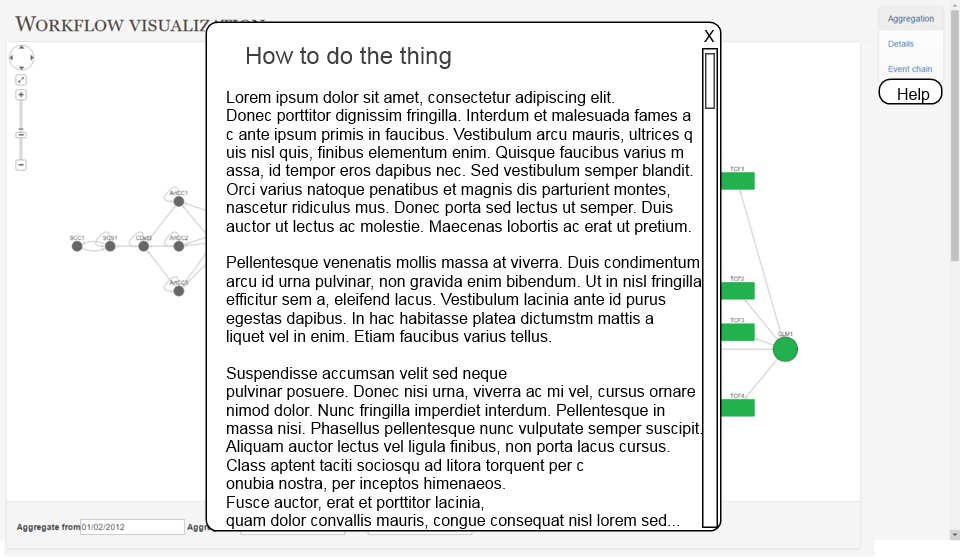
\includegraphics[scale=0.55]{pt_help_sebastian}
  \caption{En av prototyperna gjord av en gruppmedlem enligt uppgiften.}
  \label{fig:pt_help_prototype_example}
\end{figure}
\ \\
Själva rutan hade fem personer valt att göra den relativt stor så att den täckte större delen av grafen. Ett exempel kan ses i figur \ref{fig:pt_help_prototype_example}. De andra två hade gjort en mindre ruta där den ena låg ute i kanten under menyknapparna och den andra låg i grafen. Den sistnämnda var en aning tvetydig då rutan innehöll en beskrivning om att den skulle ligga i mitten av bilden, men den ändå var placerad lite till vänster i den undre halvan av bilden, se figur \ref{fig:pt_help_daniel}. Fyra prototyper beskrev att bakgrunden görs otydlig på olika sätt när hjälprutan dyker upp, till exempel genom att göra bakgrunden mörkare, oskarp, eller dimmig. Två av hjälprutorna var svagt transparenta, medan de resterande fem var täckande.
\\ \\
För stängningen av rutan hade fyra personer valt att placera ett kryss uppe i högra hörnet av rutan, vilket kan tolkas som en möjlighet att stänga rutan. Däremot hade ingen av dem explicit beskrivit om rutan kan stängas på något sätt. En av prototypernas hjälpruta stängs genom att klicka utanför rutan. Två prototyper saknar helt information om hur rutan stängs.
\\ \\
Endast en prototyp hade funktionalitet att rutan förändrar sitt innehåll beroende på vilken vy som användaren befinner sig i när hjälpknappen trycks. Ingen prototyp beskrev vad som händer om användaren byter vy medan hjälprutan är öppen. 

\subsection{Svar från enkät}
Svar på alla frågor finns att läsa i sin helhet i \ref{cha:prototyper_enkat_resultat}. När deltagarna fick jämföra sin egen prototyp mot de olika versionerna av hjälpknappen och hjälprutan tyckte de flesta att den tredje och sista versionen var mest lik deras egen prototyp. Det var också flest som var nöjda med den sista versionen. 

\begin{table}[H]
	\caption{Medelvärdet för överensstämmelse och nöjdhet över de olika versionerna av hjälpruta.}
  \def\arraystretch{1.5}
  \begin{adjustbox}{max width=\textwidth}
    \begin{tabularx}{\textwidth}{ | X | r | r |}
      \hline
      \textbf{Version} & \textbf{Överensstämmelse} & \textbf{Nöjdhet} \\
      \hline
      1 & 2 & 2,4 \\
      \hline
      2 & 2,7 & 3 \\
      \hline 
      3 & 4,1 & 4,1 \\
      \hline 
    \end{tabularx}
  \end{adjustbox}
  \label{tab:medelvarde_hjalp}
\end{table}
\ \\
Både överensstämmelsen och nöjdheten ökade för varje version, vilket kan ses i tabell \ref{tab:medelvarde_hjalp}. I svaren för både överenskommelse och nöjdhet kan man dock se att spridningen av val gick från att de flesta gav ett lågt värde på första versionen, andra versionen fick en större spridning på svaren, och tredje versionen hade flest svar på de högsta alternativen.
\\ \\
Gällande tabellen verkade de flesta i gruppen vara överens om att prototypen stämde ganska bra med deras initiala bild av den. De flesta verkade också nöjda med prototypens utseende. På samma sätt för hjälprutan var det också hög överensstämmelse och nöjdhet för den sista versionen av tabellen.

\begin{table}[h!]
	\caption{Medelvärdet för överensstämmelse och nöjdhet över de olika versionerna av tabell.}
  \def\arraystretch{1.5}
  \begin{adjustbox}{max width=\textwidth}
    \begin{tabularx}{\textwidth}{ | X | r | r |}
      \hline
      \textbf{Version} & \textbf{Överensstämmelse} & \textbf{Nöjdhet} \\
      \hline
      Prototyp & 3,7 & 4 \\
      \hline
      1 & 3,2 & 2,7 \\
      \hline 
      2 & 4,1 & 4,6 \\
      \hline 
    \end{tabularx}
  \end{adjustbox}
  \label{tab:medelvarde_tabell}
\end{table}
\ \\
Även här ökade både överensstämmelse och nöjdhet från första till andra version, vilket visas i tabell \ref{tab:medelvarde_tabell}. Däremot var medelvärdena högre för prototypen än för version ett, men bäst värden hade version två. För version ett var spridningen mellan svaren störst för både överensstämmelse och nöjdhet. Minst spridning hade version två. 
\\ \\
Tre personer i gruppen uppgav att de har fått göra om delar i gränssnittet på grund av att andra i gruppen inte har haft samma bild av slutresultatet. Alla tyckte att det har underlättat utvecklingen att ha prototyper att jobba efter, tre personer angav betyg 4 av 5 och fyra personer gav högsta betyg.
Förklaringar för hur det har underlättat att ha prototyper angavs som att det finns en bild av målet som hela gruppen kan enas kring, och att man vet när man är klar. Det angavs också att det blir en kortare utvecklingstid om det finns en målbild. Förutom det tyckte en person också att en prototyp kan agera diskussionsunderlag till fortsatt prototypande. 
\\ \\
De flesta tyckte att tiden som spenderats på att ta fram prototyper har varit väl spenderad tid. Majoriteten av gruppen tyckte också att gruppen skulle ha tagit fram prototyper för fler delar av användargränssnittet. Endast en person tyckte att prototyperna skulle utvecklats mer, resten av gruppen tyckte att detaljeringsgraden har varit lagom. Ingen tyckte att gruppen skulle tagit fram färre eller mindre utvecklade prototyper. 
\\ \\
Övriga kommentarer innehöll två svar, där deltagarna tyckte att prototyper är ett bra verktyg för att få en gemensam målbild, och också bra för att få fram andras åsikter så att fler perspektiv kan tas i beaktande.

\section{Diskussion}
\label{cha:rebecca-discussion}
I detta avsnitt diskuteras metod och resultat samt kring hur studien hade kunnat göras annorlunda. 
\subsection{Resultat}
\label{sec:rebecca-discussion-results}
Enligt Warfei \cite{prototyping-guide}, riskerar medlemmar i en utvecklingsgrupp att skapa varsin mental bild av ett system vid en textbaserad beskrivning. Detta stämmer bra överens med resultatet från den första uppgiften. Gruppmedlemmarna fick endast den textbaserade beskrivningen i  \ref{cha:gruppens_skisser}, och enligt resultatet skiljer sig alla prototyper åt. Gruppen fick uppgiften strax innan hjälprutan färdigställdes, och trots att uppgiften beskrev att prototypen skulle ritas med så lite påverkan från andra som möjligt riskerar gruppmedlemmarna ändå att ha påverkats omedvetet. Trots detta är resultaten väldigt olika, och tyder på att gruppen ännu inte hade funnit en gemensam bild, trots att en längre period av utveckling pågått.
\\ \\
Att studiens resultat stämmer överens med kunskap från teoriavsnittet syns på flera olika sätt. Svaren på fråga sju från enkäten visar på att alla gruppmedlemmar tyckte att utvecklingsarbetet förenklades av att ha prototyper att utgå från. Det faktum att hjälpknappen och hjälprutan tog tre försök för att få ett resultat där gruppen blev nöjd, jämfört med tabellens två försök tyder på att mindre arbete behövde kastas bort då en prototyp användes. Dessutom har första versionen av tabellen ett högre värde på överensstämmelse än både version ett och två av hjälprutan. Detta kan tyda på att gruppen snabbare nådde konsensus över tabellen än över hjälprutan.
\\ \\
De tre personer som har angett att de har varit tvungna att göra om delar av gränssnittet på grund av andra gruppmedlemmars åsikt har inte fått ange vilken eller vilka delar som de omarbetade. Därför kan inga slutsatser dras exakt från dessa svar. Däremot är det rimligt att åtminstone några personer bör ha fått göra om sitt arbete under projektets gång. Detta eftersom det fanns delar av användargränssnittet som saknade prototyper att utgå från, och att det enligt teoriavsnittet är större chans att en grupp saknar en gemensam bild om prototyper inte har använts. Dessutom anges även i avsnitt \ref{sec:discussion-prototyping} att en bra tidsplanering saknats, och att det har sinkat skapandet och användandet av prototyper i utvecklingen.

\subsection{Metod}
\label{sec:rebecca-discussion-method}
Studien är utförd på ett mycket litet antal personer, och kan därför göra att den är mindre trovärdig. För att få ett trovärdigt resultat hade en betydligt större undersökningsgrupp krävts. Dessutom skulle studien vara svår att återskapa exakt, då stor del av resultatet beror på individers upplevelser och tolkningar. Däremot skulle möjligen liknande resultat i avseendet skillnader på gruppmedlemmarnas prototyper kunna fås, då alla människor skapar olika mentala bilder av saker. 
\\ \\
Valet av de delar av användargränssnittet som jämfördes i studien hade kunnat göras tidigt i projektet.
Det hade gett bättre möjligheter att få mer data från de utvalda delarna, till exempel genom att isolera dem i separata utvecklingsgrenar som sedan behållits. 
Då hade kodändringarna för varje del kunnat mätas och jämföras.
Möjligheten hade också funnits att välja delar av applikationen som var mer lika varandra för att få en mer rättvis jämförelse. 
De flesta är bekanta med tabeller och vet hur de burkar se ut och hanteras. Det finns många fler sätt att utforma en hjälpruta, vilket kan ha påverkat i hur deltagarna besvarade enkäten.

\section{Slutsatser}
\label{cha:rebecca-conclusion}

\subsection{Frågeställning 1}
\textbf{Hur kan prototyper förenkla utvecklingsarbetet för en grupp?}
\\
De slutsatser som kan dras från denna studie är att prototyper kan förenkla utvecklingsarbetet för en grupp genom att finnas som en grund att utgå från. Om denna grund finns kommer gruppen uppleva arbetet som överenskommet och enklare. Prototyper minskar också risken för att arbete behöver göras om. 
\subsection{Frågeställning 2}
\textbf{Hur kan prototyper underlätta för gruppen att komma överens?}
\\
Prototyper kan också hjälpa en grupp att komma överens genom att användas som ett verktyg för att ta fram allas grafiska tolkningar av en textbaserad beskrivning. Genom att gruppen utför prototypningsarbetet tillsammans kan en gemensam bild av målet skapas som hela gruppen är nöjd med.
\subsection{Frågeställning 3}
\textbf{Kan prototyper spara tid i utvecklingsarbetet?}
\\
Om prototyper saknas riskerar en grupp att spendera mer tid än nödvändigt på att ta fram flera versioner av ett användargränssnitt. Gruppen riskerar att slösa bort sina resurser genom att behöva kassera arbete som inte motsvarar förväntningarna hos en majoritet av gruppmedlemmarna.
\\ \\
Däremot är det svårt att från denna studie dra en slutsats om prototyper kan spara tid i utvecklingsarbetet. Då väldigt lite tid skiljde utvecklingen av de olika delarna åt kan inte denna fråga besvaras med säkerhet. Denna tid är dessutom endast beräknad för utvecklingstiden och har inte tagit prototypningstid i beaktande. En förändring av metoden så som nämnts i avsnitt \ref{sec:rebecca-discussion-method} hade möjligen kunnat leda till att en slutsats hade kunnat dras. 
